
\section{Zielsetzung}
In diesem Versuch wird die Reichweite von $\alpha$-Strahlung und die Statistik des radioaktiven Zerfalls von
Americium untersucht.
\section{Theorie}
Die Entstehung von $\alpha$-Strahlung wird quantenmechanik betrachtet. Durch die gleichzeitig wirkenden Kernkräfte und
Abstoßungskräfte der Protonen ensteht ein unendlich tiefer Potentialtopf. Durch die quantenmechanische Erklärung des
Tunneleffekts können $\alpha$-Teilchen aus dem Atomkern ermittiert werden.
\newline
Dringt $\alpha$-Strahlung in Materie ein, kommt es durch Wechselwirkungen zur Energieabgabe. Zu den Wechselwirkungsprozessen
gehören die Rutherford Streuung, also die elastischen Stöße der $\alpha$-Teilchen mit der Materie, und Ionisations- und Absorptionsprozesse.
In diesem Versuch werden besonders die Ionisations- und Absorptionsprozesse betrachtet, die Rutherford Streuung spielt hierbei nur eine
untergeordnete Rolle.
\newline
Der Energieverlust ist abhängig von der Energie der $\alpha$-Strahlung und der Dichte des Materials.
Für kleine Geschwindigkeiten nimmt die Anzahl der Wechselwirkungen zu.
Die Bethe-Bloch-Gleichung beschreibt die Energieabnahme der $\alpha$-Teilchen pro Weglängeneinheit bei hinreichend großen Energien
\begin{equation}
 -\frac{dE_{\alpha}}{dx} = \frac{z^2e^4}{4\pi\epsilon_0 m_e}\frac{nZ}{\nu^2}ln\bigg(\frac{2m_e \nu^2}{I}\bigg),
\end{equation}
abhängig von der Ladung $z$ und der Geschwindigkeit $v$ der $\alpha$-Strahlung,
Ordnungszahl $Z$, der Teilchendichte $n$ und der Ionisierungsenergie $I$ des Targetgases.
Für $\alpha$-Teilchen mit sehr kleinen Energien verliert sie aufgrund der stattfindenen Ladungsaustauschprozesse
ihre Gültigkeit.
\newline
Die Reicheweite eines $\alpha$-Teilchens wird durch das Integral
\begin{equation}
 R = \int_{0}^{E_{\alpha}} \frac{dE_{\alpha}}{-dE_{\alpha}/dx}
\end{equation}
bestimmt. Dies beschreibt die Entfernung bis zu vollständigen Abbremsung der $\alpha$-Teilchen.
Die mittlere Reichweite hingegen ist die Entfernung, die noch die Hälfte der vorhandenen $\alpha$-Teilchen erreicht
\begin{equation}
  R_m = 3,1 \cdot E_{\alpha}^{\frac{3}{2}}.
  \label{eqn:Rm}
\end{equation}
Für die druckabhängige Reichweite von $\alpha$-Teilchen in Gasen gilt der folgende Zusammenhang
\begin{equation}
  x = x_0 \frac{p}{p_0}.
  \label{eqn:eff}
\end{equation}
Hierbei entspricht $x_0$ dem festen Abstand zwischen Detektor und $\alpha$-Strahler und $p_0$ dem Atmospärendruck
von 1013\,mbar.
\section{Aufbau}
Der Versuchsaufbau ist in Abbildung \ref{fig:aufbau} dargestellt.
\begin{figure}
  \centering
  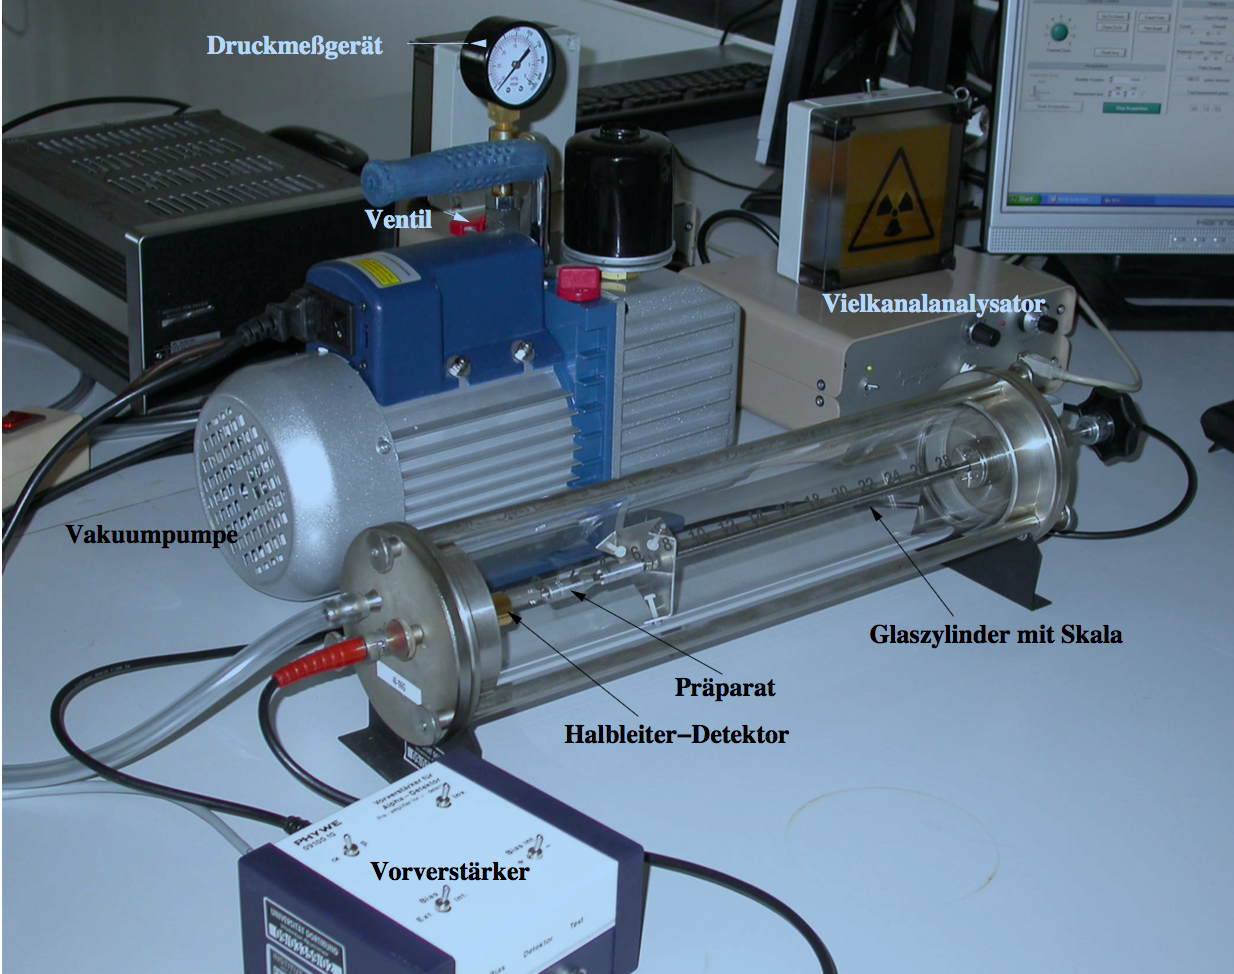
\includegraphics[scale=0.4]{aufbau.png}
  \caption{Experimenteller Aufbau.\cite{anleitung}}
  \label{fig:aufbau}
\end{figure}
\newline
Benötigt werden eine $\alpha$-Strahlungsquelle, für diesen Versuch Americium %$\ce{^{241}_{95}Am} \par$$
und einen Halbleiter-Sperrschichtzähler als Detektor in einem Glaszylinder. Der Sperrschichtzähler erzeugt bei niedriegen Energien durch einfallende
Ion Elektronen-Loch-Paare, die dann zu einem Stromimpuls im Halbleiter führen. Diese Impulse werden von einem Vorverstärker verstärkt und von einem
Vielkanalanalysator analysiert. Im Computerprogramm Multichannel Analyzer werden die unterschiedlichen Pulshöhen in einem Histogramm dargestellt.

\section{Durchführung}
Zu Beginn des Versuchs wird der Glaszylinder evakuiert. Danach werden für die zwei Abstände $x=1,5\,\mathrm{cm}$ und $x=2\,\mathrm{cm}$
für eine Minute die gemessen Counts notiert. Die gleiche Messung wird bei Atmospährendruck durchgeführt.
\newline
Bei $0\,\mathrm{mbar}$ wird die Annahme gemacht, dass die detektierte $\alpha$-Strahlung eine Energie von 4\,MeV hat.
Durch das Öffnen und Schließen der Belüftungsventils kann schrittweise der Druck um $50\,\mathrm{mbar}$ erhöht. Bis 1000\,mbar wird
jeweils für 2 Minuten die Messung durchgeführt. An Messwerten aufgenommen wird dabei Gesamtzählrate, sowie die Position des Maximums.
\newline
Zur Bestimmung der Statistik des radioaktiven Zerfalls werden im evakuierten Zylinder die Counts 100 Mal für 10 Sekunden gemessen.
